\section{Base Station Interface}
\label{sec:base-station-interface}

The Base Station serves as the primary Command and Control (C2) node for the Loon-E ASV. It provides the operator with real-time telemetry, mission status, and manual override capabilities.

\subsection{GUI Overview}
The functional prototype of the interface (Figure \ref{fig:gui-prototype}) is designed for high-glanceability during field operations. 

\begin{figure}[H]
    \centering
    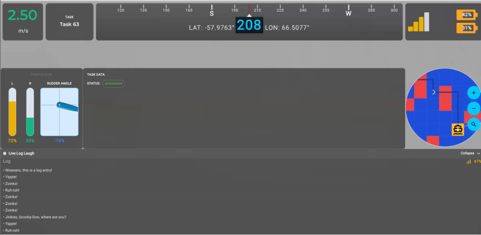
\includegraphics[width=1.0\textwidth]{images/Functional_GUI_Prototype.png}
    \caption{Functional GUI Prototype showing velocity (2.50 m/s), heading (208$^{\circ}$), and real-time path visualization.}
    \label{fig:gui-prototype}
\end{figure}

The interface includes a live log stream, battery voltage indicators for the dual-power system, and a local occupancy grid map that mirrors the data generated by the \texttt{Map Node} on the Jetson Orin Nano. This synchronization is handled via ROS2 topics bridged over the TP-Link EAP-225 communications link.